This test case repeats the exercise from Case~1c using a vulnerability model with nonzero coefficients of variation, and using four `steps\_per\_interval'. Each interval between the loss ratios specified in the vulnerability model is further divided into four equal subdivisions, thus ensuring a greater number of loss values at which the exceedance curve will be computed. For instance, the interval between the loss ratios $[0.10, 0.20]$ is now subdivided into the following loss ratios: $[0.100, 0.125, 0.150, 0.175, 0.200]$.

The loss curve thus calculated above is compared with the loss curve obtained using the OpenQuake classical PSHA based risk calculator in Figure~\ref{fig:lc-cr-1e}.

\begin{figure}[htbp]
\centering
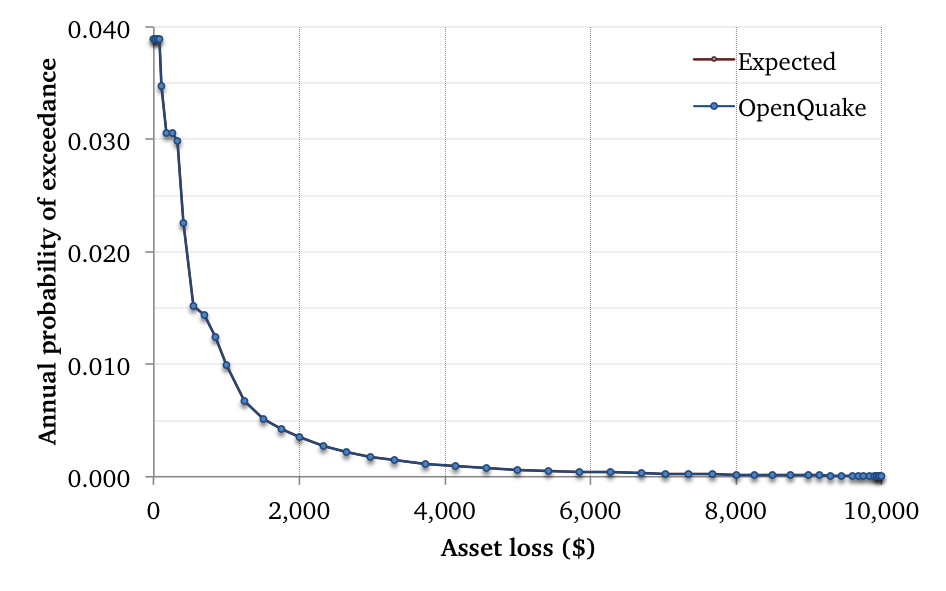
\includegraphics[width=12cm]{qareport/figures/fig-lc-cr-1e}
\caption{Loss curve comparison for classical risk test case 1e}
\label{fig:lc-cr-1e}
\end{figure}

The area under the annual loss exceedance curve gives the average annual loss.